\begin{frame}{Gradient Clipping}
	\begin{itemize}
		\item What will happen in case of a large gradient value?
		\item The gradient descent will take us \tc{keywords}{far away} from our local position.
	\end{itemize}
	\begin{figure}[H]
		\centering
		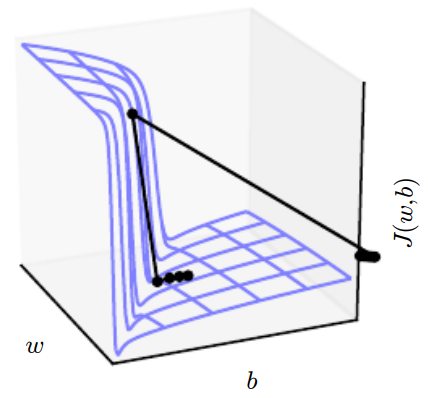
\includegraphics[width=0.4\textwidth]{Figs/gard-clipping-1.png}
		\caption{The problem of large gradient value \cite{Goodfellow-et-al-2016}.}
	\end{figure}
\end{frame}

\begin{frame}{Gradient Clipping}
	\begin{itemize}
		\item Solve this problem simply by clipping gradient.
		\item Two approaches to do so:
		\begin{itemize}
			\item Clipping by value
			\item Clipping by norm
		\end{itemize} 
	\end{itemize}
	\begin{figure}[H]
		\centering
		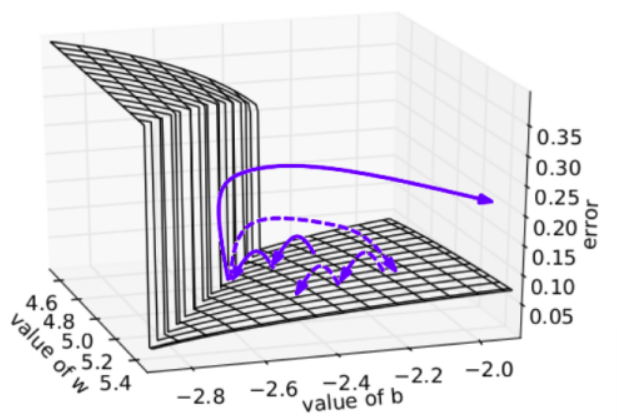
\includegraphics[width=0.5\textwidth]{Figs/clipping_more.png}
		\caption{The effect of gradient clipping. Instead of solid line\\following dotted line will lead us to minimum, \href{https://neptune.ai/blog/understanding-gradient-clipping-and-how-it-can-fix-exploding-gradients-problem}{Source}}
	\end{figure}
\end{frame}

\begin{frame}{Gradient Clipping by value}
	\begin{itemize}
		\item Set a max ($\alpha$) and min ($\beta$) threshold value.
		\item For each index of gradient $\bm{g}_i$ if it is lower or greater than your threshold clip it:
		\begin{columns}
			\centering
			\begin{column}{0.3\textwidth}
				\centering
				\[
				\begin{aligned}
					&\text{if} \; \bm{g}_i > \alpha: \\
					&\qquad \bm{g}_i \gets \alpha \\
					&\text{else if} \; \bm{g}_i < \beta: \\
					&\qquad \bm{g}_i \gets \beta
				\end{aligned}
				\]
			\end{column}
			\begin{column}{0.45\textwidth}
				\centering
				\begin{figure}[H]
					\centering	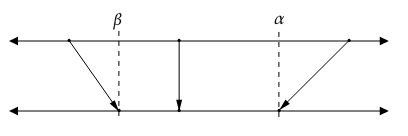
\includegraphics[width=0.95\textwidth]{Figs/clipping-value.png}
				\end{figure}
			\end{column}
		\end{columns}
	\end{itemize}
\end{frame}

\begin{frame}{Gradient Clipping by value}
	\begin{figure}[H]
		\centering
		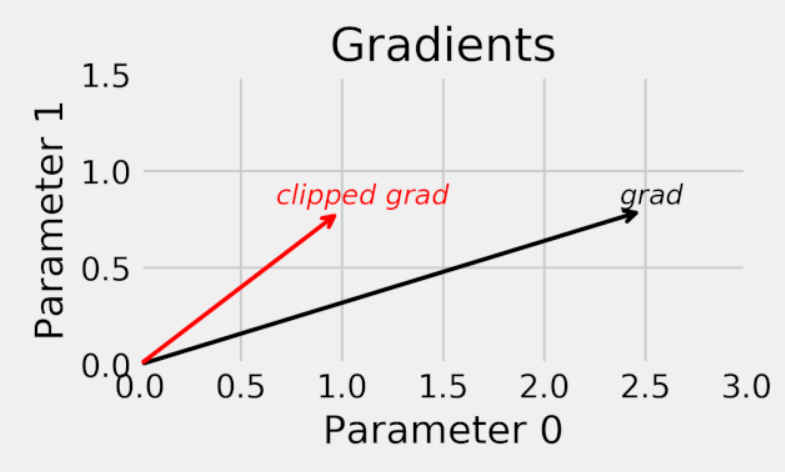
\includegraphics[width=0.5\textwidth]{Figs/clip-by-value.png}
		\caption{The effect of clipping by value. \href{https://github.com/dvgodoy/PyTorchStepByStep/blob/master/ChapterExtra.ipynb}{Source}}
	\end{figure}
	\begin{itemize}
		\item Clipping by value \tc{keywords}{will change gradient direction}.
		\item To preserve direction use clipping by norm.
	\end{itemize}
\end{frame}

\begin{frame}{Gradient Clipping by norm}
	\begin{itemize}
		\item Clip the norm $\|\bm{g}\|$ of the gradient $\bm{g}$ before updating parameters:
		\item[]
		\begin{columns}
			\centering
			\begin{column}{0.4\textwidth}
				\centering
				\[
				\begin{aligned}
					&\text{if} \; \|\bm{g}\| > v:\\
					&\qquad \bm{g} \gets \frac{\bm g}{\|\bm g\|} v
				\end{aligned}
				\]
			\end{column}
			\begin{column}{0.6\textwidth}
				\begin{figure}[H]
					\centering	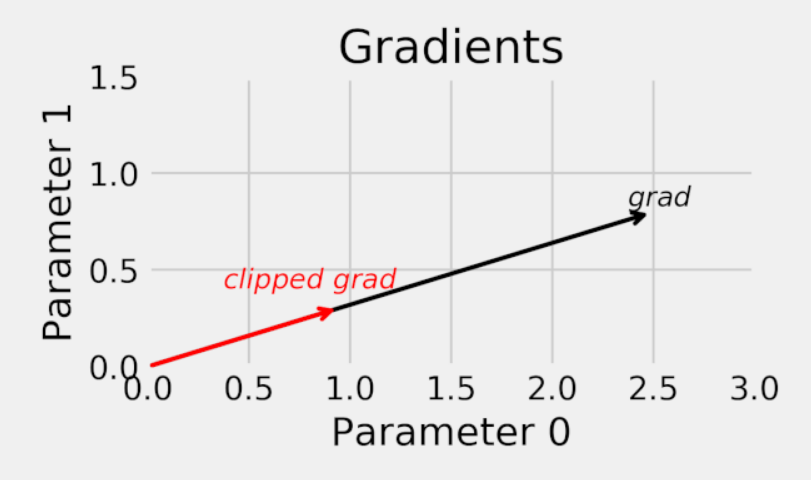
\includegraphics[width=0.65\textwidth]{Figs/clip-by-norm.png}
					\caption{The effect of clipping by norm. \href{https://github.com/dvgodoy/PyTorchStepByStep/blob/master/ChapterExtra.ipynb}{source}}
				\end{figure}
			\end{column}
		\end{columns}
		
		$v$ is the threshold for clipping which is a hyperparameter.
		\item Gradient clipping saves the direction of gradient and controls its norm.
	\end{itemize}
\end{frame}

\begin{frame}{Gradient Clipping}
	\begin{itemize}
		\item Clipping by \tc{keywords}{value} will \tc{keywords}{change the direction} of the gradient, so it will send us to a bad neighborhood.
		\item Clipping by \tc{keywords}{norm} will \tc{keywords}{preserve the direction} and just control the value.
		\item So it is better to use clipping by \tc{keywords}{norm}.
	\end{itemize}
	\begin{figure}[H]
		\centering
		\begin{subfigure}[b]{0.45\textwidth}
			\centering
			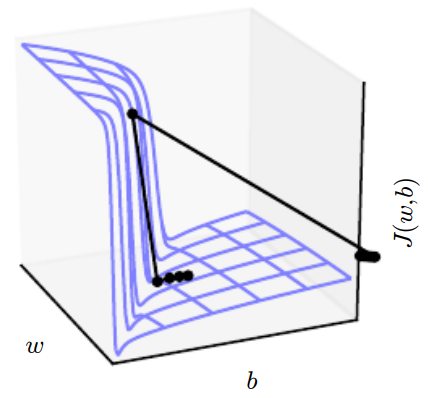
\includegraphics[width=0.75\textwidth]{Figs/gard-clipping-1.png}
		\end{subfigure}
		\begin{subfigure}[b]{0.45\textwidth}
			\centering
			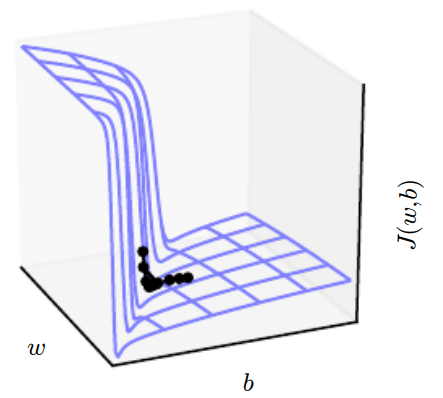
\includegraphics[width=0.75\textwidth]{Figs/grad-clipping-2.png}
		\end{subfigure}
		\caption{The "cliffs" landscape (left) without gradient clipping\\ and (right) with gradient clipping \cite{Goodfellow-et-al-2016}.}
	\end{figure}
\end{frame}